\documentclass[
	article,
	11pt,
	oneside,
	a4paper,
	english,
	brazil,
	sumario=tradicional
	]{abntex2}

\usepackage{lmodern}
\usepackage[T1]{fontenc}
\usepackage[utf8]{inputenc}
\usepackage{indentfirst}
\usepackage{nomencl}
\usepackage{color}
\usepackage{graphicx}
\usepackage{microtype}
\usepackage[brazilian,hyperpageref]{backref}
\usepackage[alf]{abntex2cite}
\usepackage[makeroom]{cancel}
\usepackage{amsmath, amssymb}
\usepackage{mathtools}
\usepackage{esint}
\usepackage{soul}
\graphicspath{{img/}}

\newcommand{\norm}[1]{\left\lVert#1\right\rVert}
\renewcommand{\backrefpagesname}{Citado na(s) página(s):~}
\renewcommand{\backref}{}
\renewcommand*{\backrefalt}[4]{
	\ifcase #1
		Nenhuma citação no texto.
	\or
		Citado na página #2.
	\else
		Citado #1 vezes nas páginas #2.
	\fi}

\titulo{Projeto 03 - Anel Carregado}
\tituloestrangeiro{}

\autor{Equipe Donner
\\[0.5cm]
Diogo Silva, Guilherme Shimada, Leonardo Vieira, Lucca Miranda, Pedro Azevedo}

\local{Brasil}
\data{17 de Novembro, 2021}

% alterando o aspecto da cor azul
\definecolor{blue}{RGB}{41,5,195}

\makeatletter
\hypersetup{
	pdftitle={\@title},
	pdfauthor={\@author},
	pdfsubject={Modelo de artigo científico com abnTeX2},
	pdfcreator={LaTeX with abnTeX2},
	pdfkeywords={abnt}{latex}{abntex}{abntex2}{atigo científico},
	colorlinks=true,
	linkcolor=blue,
	citecolor=blue,
	filecolor=magenta,
	urlcolor=blue,
	bookmarksdepth=4
}

\makeatother
\makeindex
\setlrmarginsandblock{1.5cm}{1.5cm}{*}
\setulmarginsandblock{1.5cm}{1.5cm}{*}
\checkandfixthelayout

\setlength{\parindent}{1.3cm}
\setlength{\parskip}{0.2cm}
\setlength{\columnsep}{1.0 cm}
\SingleSpacing

\begin{document}

\selectlanguage{brazil}
\frenchspacing

\twocolumn[ % INICIO DE ARTIGO EM DUAS COLUNAS
\maketitle

\begin{resumoumacoluna}

Este artigo apresenta uma discussão teórica sobre o comportamento de um anel de material isolante carregado e imerso em um campo magnético variável. Para esse propósito, foram utilizadas equações para descrever o corpo nesse ambiente, a fim de melhor compreender a mecânica dessa situação.

% \vspace{\onelineskip}

 \noindent
 \textbf{Palavras-chave}: anel carregado, rotação, momento angular, campo magnético, solenoide.
\end{resumoumacoluna}

\vspace{\onelineskip}
] % FIM DE ARTIGO EM DUAS COLUNAS

\textual
\section{Introdução}

A situação analisada neste trabalho muito se assemelha ao famoso Paradoxo Feynman, pois ela demonstra que alterações na corrente que atravessa um condutor podem causar mudanças (a princípio) contra-intuitivas no momento angular de outros corpos do mesmo sistema.

Mais especificamente, este estudo pretende analisar o efeito da interrupção da corrente que atravessa um solenoide infinito de raio $b$ sobre um anel concêntrico de raio $r \ll b$, carregado com carga $q$ e feito de material isolante. Na situação inicial, o anel está em repouso mas é livre para girar em torno de seu próprio eixo central, o qual se alinha ao eixo $z$ (vide figura \ref{campo-tangencial-img}).

A partir de uma modelagem matemática dessa situação com as equações adquiridas no decorrer da disciplina de Física Teórica III, avaliamos a resposta mecânica do anel à interrupção da corrente.

\section{Metodologia}

\subsection{O anel gira ou não gira?}
\textcolor{blue}{O momento angular inicial do sistema ($L_i$) é a soma dos momentos angulares do solenoide e do anel. O anel é feito de material isolante, então os elétrons em seu interior não se movem em relação a ele. Isso significa que, se anel está parado, assim também estão as cargas em seu interior. Portanto, o momento angular inicial provém inteiramente do movimento das cargas no interior do solenoide (lembrando que o solenoide tem a aparência de uma espiral, cujo eixo central coincide com o do anel).}

\textcolor{blue}{Quando a corrente que passa pelo solenoide é interrompida, as cargas em seu interior deixam de se mover. No entanto, o momento angular do sistema deve se conservar então as cargas no interior do anel começam a se mover. Como o anel é feito de material isolante, as cargas não se movem em relação a ele, então o anel inteiro gira.}

\textcolor{blue}{A explicação física para essa transferência de momento angular do solenoide para o anel é dada pela Lei de Lenz, que afirma que uma mudança no fluxo magnético induz o surgimento de pontecial elétrico que compensa a alteração no fluxo (esse é o significado do sinal de menos antecedendo $\Delta V$ na fórmula abaixo)}:

\begin{equation}
	\frac{d\Phi_B}{dt} = -\Delta V
\end{equation}

\textcolor{blue}{Como o campo magnético diminuiu sua componente no sentido $\hat{z}$, o campo magnético que}

\begin{equation}
	\frac{d\Phi_B}{dt} = -\Delta V = \oint_{\text{anel}} \vec{E} \cdot d\vec{l}.
\end{equation}


Quando a corrente é interrompida, o fluxo magnético sobre o anel vai de $\Phi_{Bi} = B_{\text{ext}} \pi r^2$ para $\Phi_{Bf} = 0$. Isso significa que o fluxo magnético se altera mediante o tempo, provocando o surgimento de uma tensão induzida ao redor do anel, de acordo com a Lei de Faraday:


Onde há tensão elétrica, certamente há também campo elétrico. Como o campo $B_{\text{ext}}$ era constante na direção axial, o campo elétrico que surge tem formato circular (pense na ``Regra da Mão da Direita''!), conforme a figura abaixo.

\begin{figure}[htb]
    \caption{Campo elétrico tangente ao anel}\label{campo-tangencial-img}
    \centering
    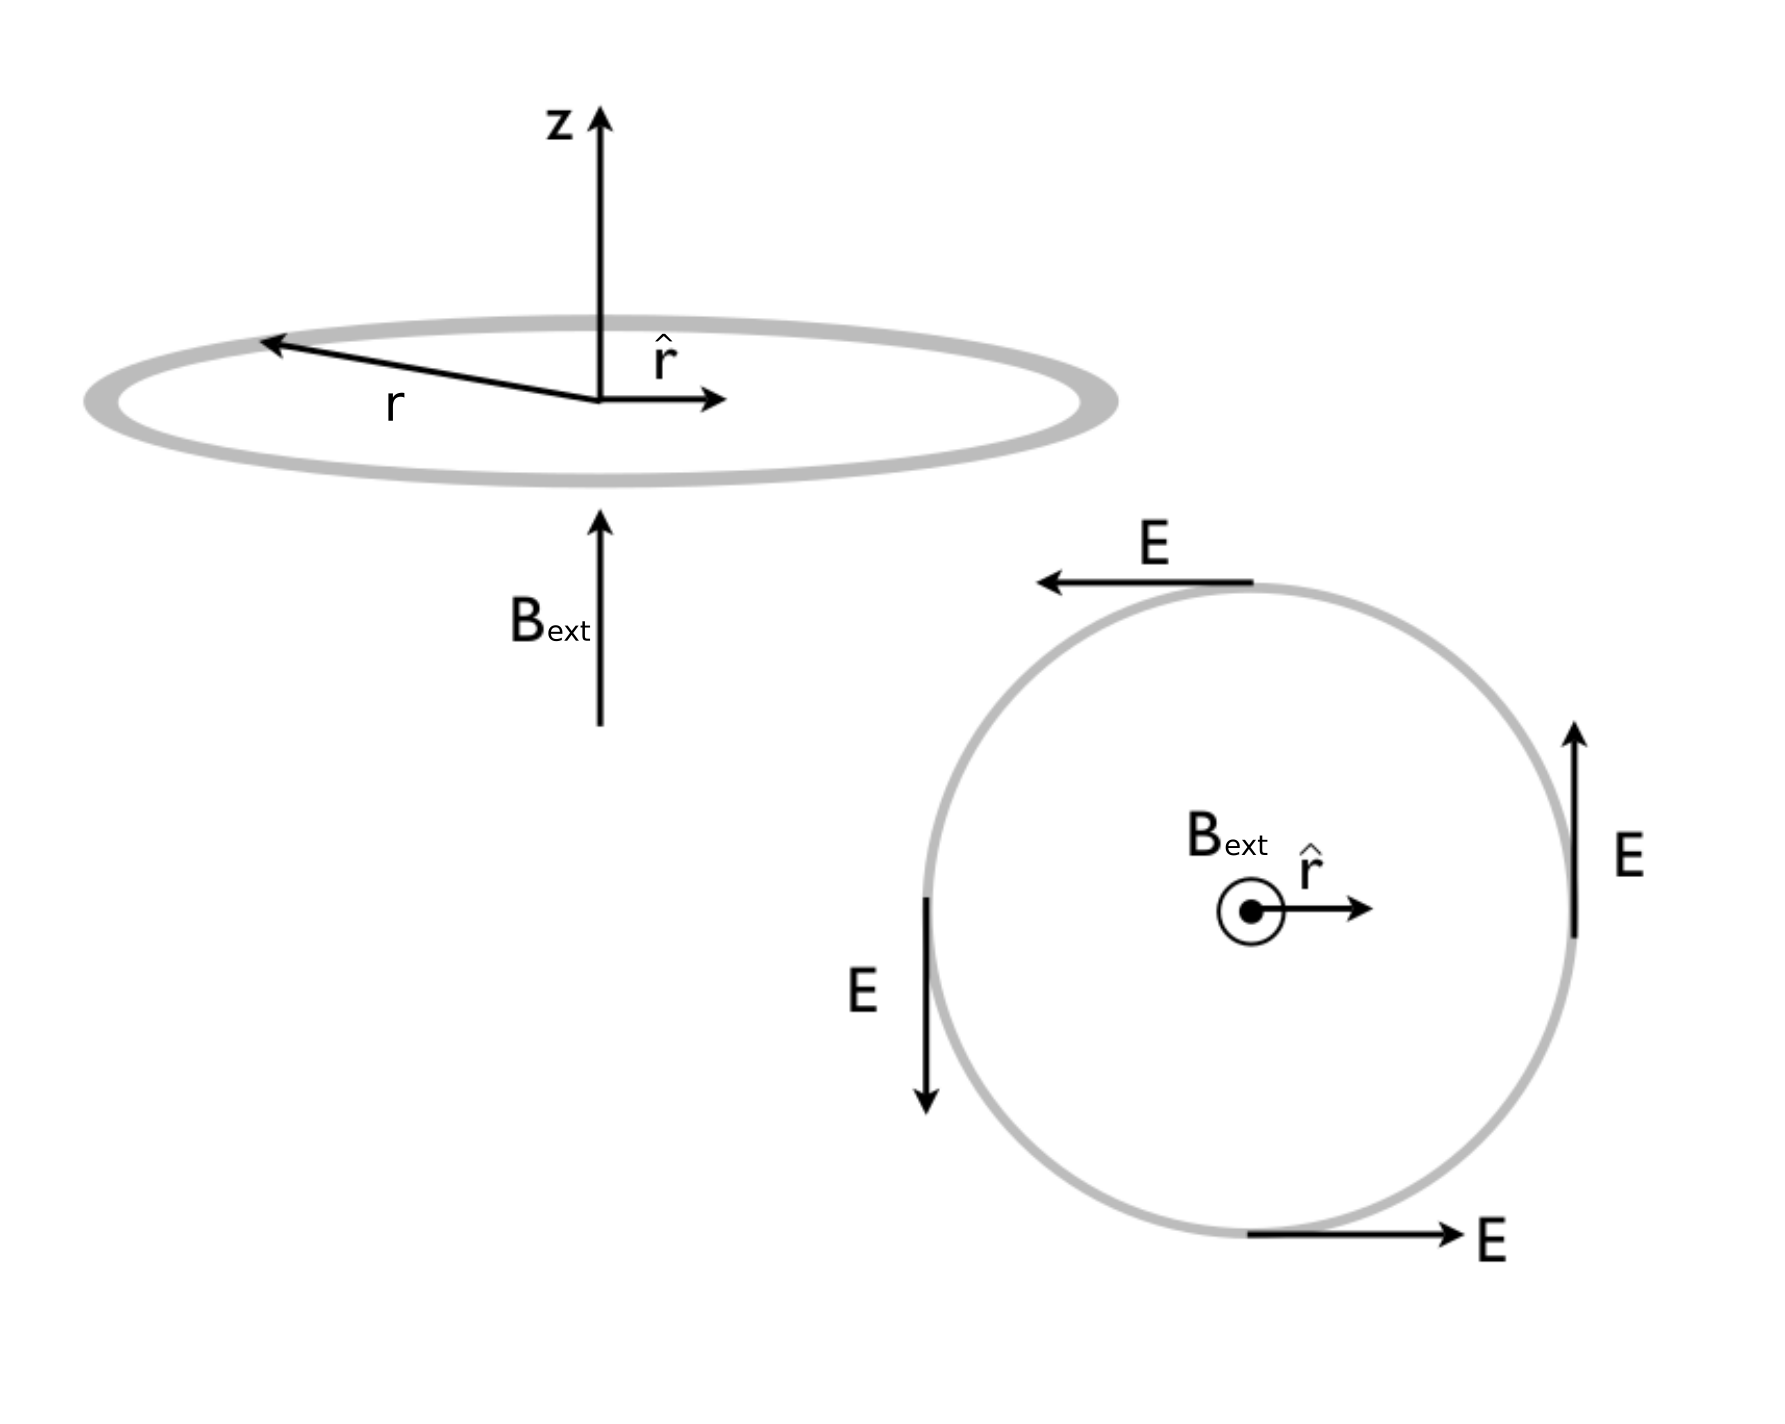
\includegraphics[width=0.4\textwidth]{corrente_tangencial.png}
	\fonte{LECLAIR, 2008}
\end{figure}

Como dito na Introdução, o anel tem um total de carga $q$ uniformemente distribuído em seu comprimento $2\pi r$, então a densidade linear de carga é $\lambda = q/(2\pi r)$ e, portanto, um elemento infinitesimal de carga é $dq = \lambda dl$. Essa notação nos permite descrever a força elétrica $d \vec{F_e}$ que surge em resposta ao campo elétrico presente em cada elemento infinitesimal de comprimento do anel como

\begin{equation} \label{lei-de-faraday-eq}
    d \vec{F_e} = dq \vec{E} = \lambda dl \vec{E}.
\end{equation}

A fim de facilitar uma compreensão mais intuitiva dessa equação (e das seguintes), incluímos uma ilustração dos elementos infinitesimais de ângulo, comprimento, e força.

\begin{figure}[htb]\label{elementos-infinitesimais-img}
    \caption{Elementos infinitesimais}
    \centering
    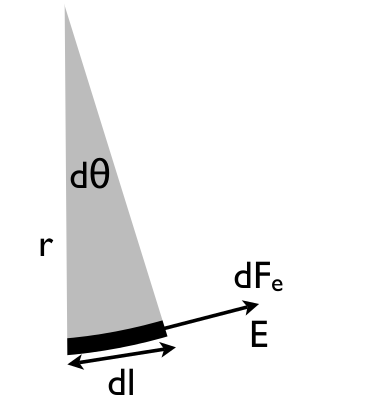
\includegraphics[width=0.3\textwidth]{elementos_infinitesimais.png}
	\fonte{LECLAIR, 2008}
\end{figure}

Essa figura ajuda a perceber que o campo elétrico tangente ao anel segue a igualdade $\vec{E} = E \hat{\theta}$, onde $\hat{\theta}$ é o versor no sentido em que o ângulo interno ao anel aumenta, logo

\begin{equation}
    d \vec{F_e} =  \lambda dl E \hat{\theta}.
\end{equation}

A partir disso, calculamos o torque em cada elemento de comprimento do anel. Como o fulcro está no centro no anel, o braço do torque equivale ao raio $\vec{r}$ do anel, então o elemento de torque é

\begin{equation}
    d \vec{\tau} = \vec{r} \times d\vec{F}
\end{equation}

\begin{equation}
    \Rightarrow d \vec{\tau} = \left(r \hat{r}\right) \times \left(\lambda dl E \hat{\theta}\right)
\end{equation}

\begin{equation} \label{elemento-de-torque-eq}
    \Rightarrow d \vec{\tau} = \lambda r dl E \left(\hat{r} \times \hat{\theta}\right).
\end{equation}

Pela ``Regra da Mão Direita'', o produto vetorial da equação \ref{elemento-de-torque-eq} equivale a $\hat{z}$ (isso é mais fácil de perceber se você der um ``tapa'' com a mão direita, do versor $\hat{r}$ para um dos vetores $\vec{E}$ na figura \ref{campo-tangencial-img}), então o elemento de torque é

\begin{equation}
    \Rightarrow d \vec{\tau} = \lambda r dl E \hat{z},
\end{equation}

\noindent e, portanto, o torque no anel inteiro é

\begin{equation}
    \vec{\tau} = \oint_{\text{anel}} d \vec{\tau} = \lambda r \left(\oint_{\text{anel}} dl E\right) \hat{z}.
\end{equation}

Como o campo elétrico é tangencial, $d\vec{l} \parallel \vec{E}$ em todo o anel. Por esse motivo temos $dl E = d\vec{l} \cdot \vec{E} $, então

\begin{equation}
    \vec{\tau} = \lambda r \left(\oint_{\text{anel}} d\vec{l} \cdot \vec{E}\right) \hat{z},
\end{equation}

\noindent que pela Lei de Faraday (vide equação \ref{lei-de-faraday-eq}) é

\begin{equation}
    \vec{\tau} = \left(\lambda r \Delta V \right) \hat{z}
\end{equation}

\begin{equation}
    \Rightarrow \vec{\tau} = \left(\frac{q}{2\pi \cancel{r}}~\cancel{r} \Delta V \right) \hat{z} = \left(\frac{q \Delta V}{2\pi}\right) \hat{z}
\end{equation}

Agora que ajeitamos todas as direções, podemos substituir a notação vetorial pela notação escalar obtendo a equação

\begin{equation}
    \tau =  \left(\frac{q \Delta V}{2\pi}\right),
\end{equation}

\noindent que, pela Lei de Faraday, equivale a

\begin{equation}
    \tau =  - \left(\frac{q}{2\pi}\right)\frac{d \Phi_B}{d t}.
\end{equation}

Note que $q \ne 0$ e $\Delta V \ne 0$, então o torque é não-nulo e, portanto, o anel gira.

\subsection{Velocidade angular do anel}
Pela Segunda Lei de Newton, o torque resultante equivale a derivada temporal do momento angular $L$, então

\begin{equation}
    \tau = \frac{dL}{dt} =  - \left(\frac{q}{2\pi}\right)\frac{d\Phi_B}{dt}
\end{equation}

\begin{equation} \label{integral-momento-angular-eq}
    \Rightarrow \int_i^f dL = \int_i^f - \left(\frac{q}{2\pi}\right) d\Phi_B,
\end{equation}

\noindent onde os limites de integração $i$ e $f$ representam os instantes imediatamente anterior e posterior ao desligamento da corrente do solenoide, respectivamente. Resolvendo as integrais da equação \ref{integral-momento-angular-eq}, obtemos

\begin{equation}
    L_f - L_i = \frac{q}{2\pi}(\Phi_{Bi} - \Phi_{Bf}).
\end{equation}

Nessa equação, $L_i = 0$ pois o anel está estacionário na situação inicial e, portanto, seu momento angular inicial é nulo. Como o anel está girando na situação final, ele gera o próprio campo magnético que, segundo a dica dada no enunciado, pode ser modelado como $B_{\text{anel}} = A\lambda\omega$. Isso significa que o momento angular final do anel é

\begin{equation}
    L_f - \cancelto{0}{L_i}= \frac{q}{2\pi}(B_{\text{ext}}\pi r^2 - B_{\text{anel}} \pi r^2)
\end{equation}

\begin{equation}
    \Rightarrow L_f = \frac{q r^2 \cancel{\pi}}{2\cancel{\pi}} (B_{\text{ext}} - B_{\text{anel}})
\end{equation}

\begin{equation}
    \Rightarrow L_f = \frac{q r^2}{2} (B_{\text{ext}} - A\lambda\omega)
\end{equation}

Sabendo que o momento de inércia $I$ de um anel de raio $r$ e massa $m$ é dado por $I = mr^2$, podemos calcular a velocidade angular $\omega$ como

\begin{equation}
    \omega = \frac{Lf}{I} = \frac{q \cancel{r^2}}{2m \cancel{r^2}}(B_{\text{ext}} - A\lambda\omega)
\end{equation}

\begin{equation}
    \Rightarrow \omega = \frac{qB_{\text{ext}}}{2m} + \frac{A\lambda\omega}{2m}
\end{equation}

\begin{equation}
    \Rightarrow \omega - \frac{A\lambda\omega}{2m} = \frac{qB_{\text{ext}}}{2m}
\end{equation}

\begin{equation}
    \Rightarrow \omega \left(1 - \frac{A\lambda}{2m} \right)= \frac{qB_{\text{ext}}}{2m}
\end{equation}

\begin{equation}
    \Rightarrow \omega \left(\frac{2m - A\lambda}{2m} \right)= \frac{qB_{\text{ext}}}{2m}
\end{equation}

\begin{equation}
    \Rightarrow \omega = \frac{qB_{\text{ext}}}{\cancel{2m}}\left(\frac{\cancel{2m}}{2m - A\lambda} \right)
\end{equation}

\begin{equation}
    \Rightarrow \boxed{\omega = \frac{qB_{\text{ext}}}{2m - A\lambda}}
\end{equation}

\subsection{Campo magnético inicial}

\textcolor{blue}{Sabemos pela Lei de Ampére (precisa deduzir?) que a fórmula do campo magnético produzido por um solenoide é dado por:}


\textcolor{blue}{\begin{equation}
    B_{\text{ext}} = \mu_0 i \left(\frac{N}{L}\right),
\end{equation}}

\noindent\textcolor{blue}{que pela definição de corrente, equivale a}

\textcolor{blue}{\begin{equation}
    B_{\text{ext}} = \mu_0 \left(\frac{Q}{\Delta t}\right) \left(\frac{N}{L}\right),
\end{equation}}

\noindent\textcolor{blue}{onde $\Delta t$ é o tempo necessário para um elétron percorrer o solenoide inteiro, de ponta a ponta (o solenoide é infinito, mas essa abstração é necessária para a demonstração). Devido ao jeito que definimos $\Delta t$, o total de carga que passa pelo solenoide nesse intervalo de tempo equivale ao total de carga contido no solenoide então:}

\textcolor{blue}{\begin{equation}
    B_{\text{ext}} = \mu_0 \left(\frac{q_e n_e \cancel{L}}{\Delta t}\right) \left(\frac{N}{\cancel{L}}\right),
\end{equation}}

\textcolor{blue}{\begin{equation}
    \Rightarrow B_{\text{ext}} = \mu_0 q_e n_e \left(\frac{N}{\Delta t}\right),
\end{equation}}

\noindent\textcolor{blue}{em que $q_e$ é a carga elementar e $n_e$ é a densidade linear de elétrons. Observe que, agora, os únicos valores desconhecidos na expressão do campo magnético do solenoide são $N$ e $\Delta t$. Para resolver isso, escrevemos esses termos em função da velocidade azimutal $v_e$ e de outros dados conhecidos:}

\textcolor{blue}{\begin{equation}
    v_e = \frac{L}{\Delta t}
\end{equation}}

\textcolor{blue}{\begin{equation}
    \Rightarrow v_e = \frac{N(2\pi b)}{\Delta t}
\end{equation}}

\textcolor{blue}{\begin{equation}
    \Rightarrow \frac{N}{\Delta t} = \frac{v_e}{2\pi b}.
\end{equation}}

\textcolor{blue}{Assim, a expressão do campo magnético gerado pelo solenoide é}

\textcolor{blue}{\begin{equation}
    \Rightarrow B_{\text{ext}} = \mu_0 q_e n_e \left(\frac{v_e}{2\pi b}\right),
\end{equation}}


\noindent\textcolor{blue}{a partir da qual podemos expressar a velocidade azimutal como}


\textcolor{blue}{\begin{equation}
    v_e = \frac{B_{\text{ext}} 2\pi b}{\mu_0 n_e q_e},
\end{equation}}

\noindent\textcolor{blue}{e, consequentemente, a velocidade angular $\omega$ como}

\textcolor{blue}{\begin{equation}
    \omega_e \cancel{b} = \frac{B_{\text{ext}} 2\pi \cancel{b}}{\mu_0 n_e q_e}
\end{equation}}

\textcolor{blue}{\begin{equation}
    \Rightarrow\omega_e = \frac{B_{\text{ext}} 2\pi}{\mu_0 n_e q_e}.
\end{equation}}

Por fim, sabendo que $\omega = L/I$ e que o momento de inércia de um cilindro oco (como é o caso do solenoide) é $I = m b^2$, temos a seguinte expressão final para o momento angular inicial:

\textcolor{blue}{\begin{equation}
    \frac{L}{m b^2} = \frac{B_{\text{ext}} 2\pi}{\mu_0 n_e q_e}
\end{equation}}

\textcolor{blue}{\begin{equation}
    \Rightarrow L = \frac{B_{\text{ext}} 2\pi~m b^2}{\mu_0 n_e q_e}
\end{equation}}





\section{Resultados e Conclusão}

Em primeira instância, é importante ressaltar que o primeiro argumento proposto no enunciada da questão que motivou essa pesquisa está correto e o anel vai girar! Além dessa conclusão, fomos capazes de determinar a velocidade angular do anel, bem como o campo magnético inicial do problema.

\nocite{leclair_2008, reville_2016}

\pagebreak
\onecolumn{
\postextual
\bibliography{references}
}

\end{document}
